\subsection{Coverage Calculation}
\begin{frame}
\frametitle{Coverage Calculation}
\begin{center}
  \begin{equation*}
    FunctionCoverage = \frac{Number of Tested Methods}{Total Number of Methods}
  \end{equation*}
\end{center}
\end{frame}

\begin{frame}
  \frametitle{Coverage Example}
  \begin{center}

  \begin{table}[htbp]
  %   \centering
   \resizebox{6.5cm}{!}{%
    \begin{tabular}{|c|c|c|c|c|c|}
      \hline
  %
      \bf NUMM     & \bf NUMTM & \bf Function Coverage \\ \hline\hline
      40  & 25  & 62.5\%  \\ \hline
  %
  %
    \end{tabular}%
    }

  \end{table}

  \end{center}
\end{frame}

\subsection{Truly-Tested-Method Calculation}
\begin{frame}
  \frametitle{Truly-Tested-Method Calculation}
  \begin{itemize}
    \item \textbf{Number of Truly-Tested-Methods = NUMTTM}

    \item \textbf{Number of Tested Methods = NUMTM}

    \item \textbf{Number of Pseudo-tested Methods = NUMPTM}
  \end{itemize}

  \begin{center}
    \begin{equation*}
      NUMTTM = NUMTM - NUMPTM
    \end{equation*}
  \end{center}
\end{frame}

\begin{frame}
  \frametitle{Truly-Tested-Method Example}
  \begin{center}

  \begin{table}[htbp]
  %   \centering
   \resizebox{6.5cm}{!}{%
    \begin{tabular}{|c|c|c|c|c|c|}
      \hline
  %
      \bf NUMTM     & \bf NUMPTM & \bf NUMTTM \\ \hline\hline
      25  & 3  & 22  \\ \hline
  %
  %
    \end{tabular}%
    }

  \end{table}

  \end{center}
\end{frame}

\begin{frame}
\frametitle{Updated-Coverage Calculation}
\begin{center}
  \begin{equation*}
    UC = \frac{Number of TrulyTested Methods}{Total Number of Methods}
  \end{equation*}
\end{center}
\end{frame}

\subsection{Metrics Produced}
\begin{frame}
  \frametitle{Output}

    \begin{figure}
    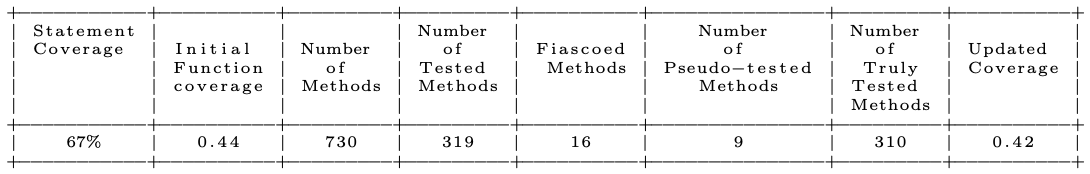
\includegraphics[scale = .55]{images/tableOutput}
    \end{figure}
\end{frame}
